\documentclass[final]{beamer}
\usepackage[scale=1.24]{beamerposter} % Use the beamerposter package for laying out the poster
\usetheme{confposter} % Use the confposter theme supplied with this template

\setbeamercolor{block title}{fg=ngreen,bg=white} % Colors of the block titles
\setbeamercolor{block body}{fg=black,bg=white} % Colors of the body of blocks
\setbeamercolor{block alerted title}{fg=white,bg=dblue!70} % Colors of the highlighted block titles
\setbeamercolor{block alerted body}{fg=black,bg=dblue!10} % Colors of the body of highlighted blocks

%-----------------------------------------------------------
% Define the column widths and overall poster size
% To set effective sepwid, onecolwid and twocolwid values, first choose how many columns you want and how much separation you want between columns
% In this template, the separation width chosen is 0.024 of the paper width and a 4-column layout
% onecolwid should therefore be (1-(# of columns+1)*sepwid)/# of columns e.g. (1-(4+1)*0.024)/4 = 0.22

\newlength{\sepwid}
\newlength{\onecolwid}

% Posters should be 90 x 122 cm in landscape orientation.
\setlength{\paperheight}{90cm}
\setlength{\paperwidth}{122cm}

% \setlength{\paperwidth}{48in} % A0 width: 46.8in
% \setlength{\paperheight}{36in} % A0 height: 33.1in

% \setlength{\paperwidth}{40in} % A0 width: 46.8in
% \setlength{\paperheight}{30in} % A0 height: 33.1in



\setlength{\sepwid}{0.02\paperwidth} % Separation width (white space) between columns
\setlength{\onecolwid}{0.22\paperwidth} % Width of one column
 % \setlength{\onecolwid}{0.32\paperwidth} % Width of one column
\setlength{\topmargin}{-0.5in} % Reduce the top margin size
%-----------------------------------------------------------

\usepackage{graphicx}  % Required for including images
\usepackage{booktabs} % Top and bottom rules for tables
\usepackage{natbib} 
 
\title{COMS W4995 Final Report: Automatic Data Augmentation Policy Selection} % Poster title
\author{Jonathan D. Armstrong, Jesse Galef, and Kyle Matoba} % Author(s)
\institute{Computer Science Department, Columbia University} % Institution(s)

\begin{document}

\addtobeamertemplate{block end}{}{\vspace*{2ex}} % White space under blocks
\addtobeamertemplate{block alerted end}{}{\vspace*{2ex}} % White space under highlighted blocks
\setlength{\belowcaptionskip}{2ex} % White space under figures
\setlength\belowdisplayshortskip{2ex} % White space under equations

\begin{frame}[t] % The whole poster is enclosed in one beamer frame
\begin{columns}[t] % The whole poster consists of three major columns, the second of which is split into two columns twice - the [t] option aligns each column's content to the top

\begin{column}{\sepwid} \end{column} % Empty spacer column
\begin{column}{\onecolwid} % The first column

\begin{alertblock}{Objectives}
  	
	
  Approach or improve upon state of the arts results in image classification on the CIFAR-10 dataset (\cite{Krizhevsky2009}) by learning data augmentation policies from data. Build on the work of AutoAugment\cite{Cubuk2018}, but with an emphasis on practical accessibility to those without supercomputing resources.
\end{alertblock}

% INTRODUCTION

\begin{block}{Introduction}

	\begin{equation}
		\text{SOTA Accuracy} = \text{SOTA Data Augmentaiton } + \text{ SOTA Model}
	\end{equation}

  The AutoAugment authors have proven that state of the art results (SOTA) can be achieved simply by using a good data augmentation policy on an already proven SOTA model. Their innovation is the use of reinforcement learning to generate this policy from the data itself. The data augmentation policies considered consist of image transforms applied homogeneously to every image category. Recognizing that each image category can have different invariants, we explored finer-grained policy architectures that support targeting transforms to each individual image category.

  %Data augmentation is indispensable for obtaining state of the art performance on image classification. For example, not only does \cite{Recht2018} find that data augmented models perform considerably much better than un-augmented models, but all of the best-performing models on the CIFAR 10 dataset include data augmentation. Furthermore, the augmented models perform better on ``CIFAR 10.1'', a recently collected secondary test set\cite{Recht2018}. , and have lower drops in accuracy between in-sample and out-of-sample accuracy.

  \begin{figure}
    \centering
    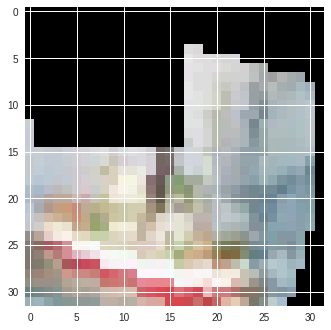
\includegraphics[width=0.70\textwidth]{ship.png}
    \caption{
    	An example of an augmented image in the CIFAR-10 dataset: a random box of pixels have been set to black (called ``cutout'', \cite{Devries2017}), it has been randomly rotated, and again had cutout applied. It is still recognizable as a ship, though its raw representation is completely different.}
    \label{fig:cutout_ship}
  \end{figure}
\end{block}

%\begin{block}{Wide ResNet}
%  \cite{Zagoruyko2016}

%\end{block}

\begin{block}{Hardware Accelerators}
  Our results were computed on Google Colaboratory with a Tensor Processing Unit backend.
  If you have an already compiled \texttt{tf.keras} model called \texttt{m} then you can convert it to a \texttt{KerasTPUModel} simply:

  {\small
    \texttt{w = 'grpc://' + os.environ['COLAB\_TPU\_ADDR']} \\
    \texttt{r = tf.contrib.cluster\_resolver.TPUClusterResolver(w)} \\
    \texttt{s = tf.contrib.tpu.TPUDistributionStrategy(r, False)} \\
    \texttt{m = tf.contrib.tpu.keras\_to\_tpu\_model(m, strategy=s)}
  }

  We saw a roughly 15 times speed up over a K80 GPU (albeit after a few minutes of compilation) on this task. 


\end{block}

\end{column} % End of the first column

\begin{column}{\onecolwid} % Begin a column which is two columns wide (column 2)
% \begin{column}{\onecolwid}\vspace{-.6in} % The second column within column 2 (column 2.2)
% \end{column} % End of column 2.2

\begin{block}{Na\"{\i}ve Analysis}

 We leveraged the concept of composition to create a simple policy. Using a basic model and $1/10$ of the training data, we established a baseline performance then evaluated how test accuracy changed for each image category when a single transform was applied. Using these results, our best performing policy ironically ignored image category information. 

 \begin{figure}
 	\centering
 	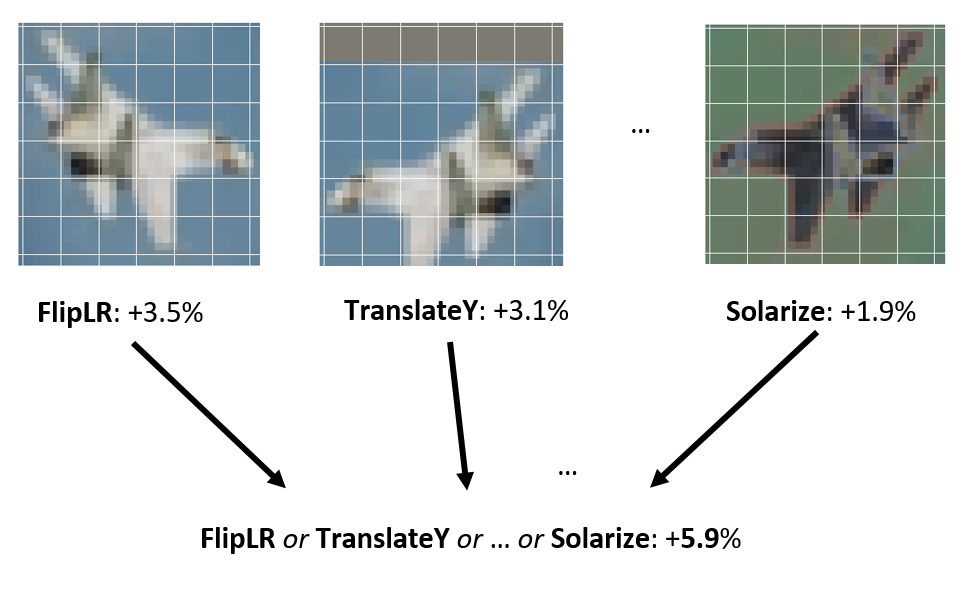
\includegraphics[width=0.70\textwidth]{naive_analysis.png}
 	\caption{
 		The best policy combined the transforms that improved performance by at least one percent then randomly selected one of these policies to apply to the images for each step of stochastic gradient descent. When combining the best individual transforms, we acheive test accuracy greater than any individual transform was able to acheive.} 
 	\label{fig:niave_analysis}
  \end{figure}

  After identifying our best na\"{\i}ve analysis policy, we evaluated its performance against AutoAugment on the state of the art Wide ResNet model \cite{Zagoruyko2016}.

  \begin{table}[h]
	\begin{tabular}{l|c|c}
		\hline
		Policy  &CIFAR-10 Test  &CIFAR-10.1 Test  \\
		&Accuracy (\%)  &Accuracy (\%) \\ \hline
		Cutout + Flipping                 & 96.10 & 91.80 \\
		AutoAugment			        & 96.98 & 92.30 \\
		Na\"{\i}ve Analysis 			&96.80	&92.40 \\
	\end{tabular}
	\caption{WRN model \cite{Zagoruyko2016} test accuracies for CIFAR-10 and CIFAR-10.1}
  \end{table}

  \textbf{Notice that we are able to approach the performance of AutoAugment (which uses a sophisticated reinforcement learning scheme) with a simple and easy to understand approach.}

  Using what we learned from this na\"{\i}ve analysis approach, can we do better?  

\end{block}



\begin{block}{Reinforcement Learning: Image Class Targeted Policies}

  We coded our own implementation of the AutoAugment procedure that supports policies with transforms at image class level. 

  \begin{figure}
	\centering
	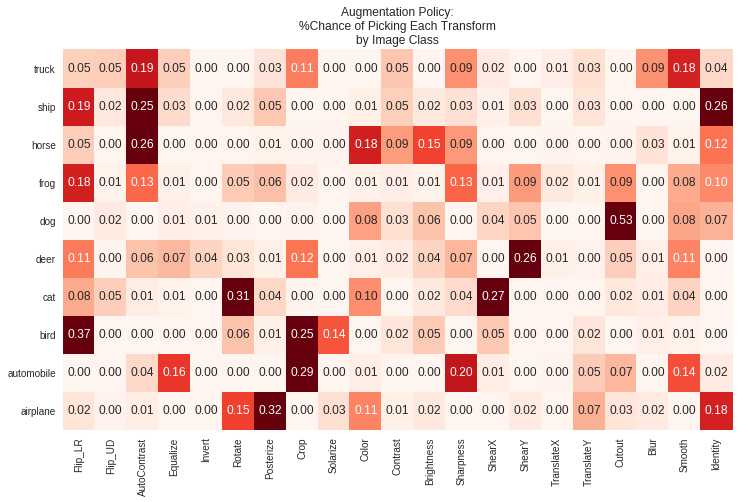
\includegraphics[width=0.70\textwidth]{splitPolicy.png}
	\caption{
		Notice how transform probabilities are far from homogeneous for each image category.}
	\label{fig:cutout_ship}
  \end{figure}

\end{block}


%\begin{block}{Fundamental bound on achievable accuracy?}

%{\small
%\texttt{import keras} \\
%\texttt{import matplotlib.pyplot as plt} \\

%\texttt{labels = ['plane', 'car', 'bird', 'cat', 'deer', 'dog', 'frog', 'horse', 'ship', 'truck']} \\
%\texttt{\_, (x, y) = keras.datasets.cifar10.load\_data()} \\
%\texttt{plt.imshow(x[2405, :, :, :])} \\
%\texttt{plt.title(labels[y[2405, 0]])}
%}

%  \begin{figure}
%  \centering
%  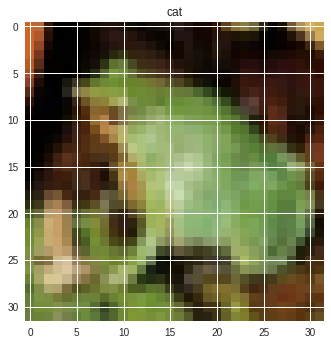
\includegraphics[width=0.70\linewidth]{catfrog.png}
%  \end{figure}


%\end{block}


% IMPORTANT RESULT
% \begin{alertblock}{Important result} 
% \end{alertblock} 

\end{column} % End of the second column

\begin{column}{\sepwid}\end{column} % Empty spacer column
\begin{column}{\onecolwid} % The third column

\begin{block}{Conclusion}
		
  We have demonstrated that very simple policy searches suffice for obtaining nearly optimal performance-enhancing image augmentation. Together with a relatively lightweight Wide ResNet fit upon a free TPU, we are able to present an at-or-near state of the art CIFAR-10 image classifier that can be fit quickly and cheaply, an increasingly important criterion (\cite{Coleman2017}).
  
  We had insufficient time to fully realize final results from our custom AutoAugment algorithm, but our initial results demonstrate that considering policy architectures at the image class level has potential. 
  
  
\end{block}

\begin{block}{References}
%\begin{spacing}{0.75}
	
	% \printbibliography
	\bibliographystyle{plainnat}  % needs package natbib
	
	\bibliography{../biblio}   
	
%\end{spacing}	
	
%{\small
%\bibliographystyle{ieee}
%\bibliography{../biblio}
%}
\end{block}

% ACKNOWLEDGEMENTS
\setbeamercolor{block title}{fg=red,bg=white} % Change the block title color
\begin{block}{Acknowledgements}
Many thanks to Professor Drori for his help and encouragement. \\
\end{block}

% CONTACT INFORMATION
\setbeamercolor{block alerted title}{fg=black,bg=norange} % Change the alert block title colors
\setbeamercolor{block alerted body}{fg=black,bg=white} % Change the alert block body colors

\begin{alertblock}{Contact Information}
\begin{itemize}
\item Jonathan: \href{mailto:jda2160@columbia.edu}{\texttt{jda2160@columbia.edu}}
\item Jesse: \href{mailto:jbg2160@columbia.edu}{\texttt{jbg2160@columbia.edu}}
\item Kyle: \href{mailto:km3227@columbia.edu}{\texttt{km3227@columbia.edu}}
\end{itemize}
\end{alertblock}

\begin{center}

\includegraphics[width=0.8\linewidth]{logo.jpg} % & \hfill & 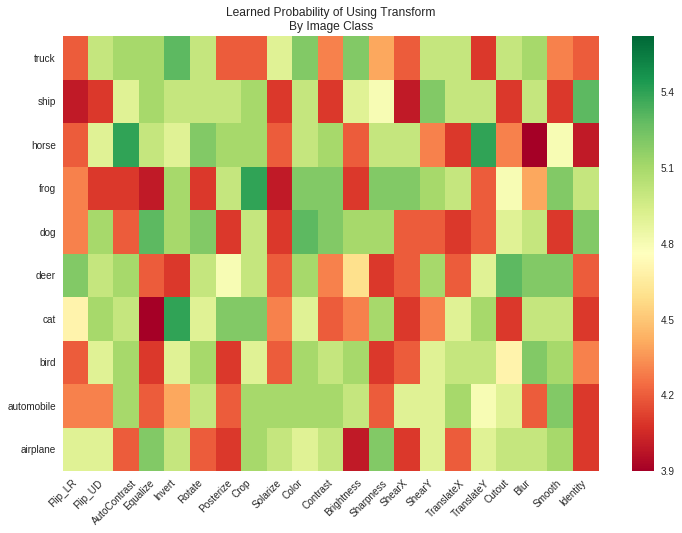
\includegraphics[width=0.4\linewidth]{logo.png}
\end{center}

\end{column} % End of the third column
\end{columns} % End of all the columns in the poster
\end{frame} % End of the enclosing frame
\end{document}
